\documentclass[11pt]{cernrep} \usepackage{graphicx,epsfig} \bibliographystyle{lesHouches}
\usepackage{xspace}
\newcommand{\Sherpa}{S\protect\scalebox{0.8}{HERPA}\xspace}
\newcommand{\CSS}{C\protect\scalebox{0.8}{SS}\xspace}
\newcommand{\Comix}{C\protect\scalebox{0.8}{OMIX}\xspace}
\newcommand{\Amegic}{A\protect\scalebox{0.8}{MEGIC++}\xspace}
\newcommand{\MCatNLO}{M\protect\scalebox{0.8}{C}@N\protect\scalebox{0.8}{LO}\xspace}
\newcommand{\MEPS}{M\scalebox{0.8}{E}P\scalebox{0.8}{S}\xspace}
\newcommand{\MEPSatNLO}{M\scalebox{0.8}{E}P\scalebox{0.8}{S}@N\protect\scalebox{0.8}{LO}\xspace}
\newcommand{\Collier}{C\protect\scalebox{0.8}{OLLIER}\xspace}
\newcommand{\OpenLoops}{O\protect\scalebox{0.8}{PEN}L\protect\scalebox{0.8}{OOPS}\xspace}
\newcommand{\Herwig}{H\protect\scalebox{0.8}{ERWIG}7\xspace}
\newcommand{\Matchbox}{M\protect\scalebox{0.8}{ATCHBOX}\xspace}
\newcommand{\MadGraph}{M\protect\scalebox{0.8}{AD}G\protect\scalebox{0.8}{RAPH}\xspace}
\newcommand{\CVolver}{CV\protect\scalebox{0.8}{OLVER}\xspace}
\newcommand{\ColorFull}{C\protect\scalebox{0.8}{OLOR}F\protect\scalebox{0.8}{ULL}\xspace}
\newcommand{\pt}{\ensuremath{p_{T}}\xspace}

\begin{document}

\section{Study of associated production of vector bosons and b-jets in
  pp collisions at the LHC \protect\footnote{Contributing authors:
    M.~Bell, J.~Butterworth,  V.~Ciulli,
    G.~Hesketh, F. ~Krauss, G.~Luisoni, G.~Nail, D.~Napoletano,
    C.~Oleari, S.~Platzer, C.~Reuschle, B.~Waugh, ... }}

\subsection{Introduction}



\subsection{Rivet Routines}

Results in this study were produced using three Rivet routines to compare to published ATLAS and CMS data.

\begin{itemize}
\item Measurement of differential production cross-sections for a $Z$\ boson in association with b-jets in proton-proton collisions at $\sqrt{s} = 7$~TeV with the ATLAS detector~\cite{Aad:2014dvb} (Rivet routine Rivet routine ATLAS\_2014\_I1306294). A pair of opposite sign charge dressed leptons\footnote{Leptons are dressed by adding the four-vectors of all photons within $\Delta R<0.1$\ to the lepton 4-vector} (i.e. electrons or muons) with $\pt>20$~GeV and $|\eta|<2.5$ are required, with a dilepton mass between 76 and 106~GeV. Anti-k$_{t}$\ 0.4 jets are reconstructed from all final state particles, and required to have $\pt>$20~GeV, $|y|<2.4$ and not overlap with the leptons used to make the $Z$~candidate ($\Delta R(jet, l)> 0.5$). Jets are labelled as $b$-jets based on matching with $\Delta  R<0.3$ to a weakly decaying $b$-hadron with $\pt>5$~GeV.

  Distributions include the \pt and rapidity of $b$-jets and of the $Z$-boson, and for each $b$-jet, the $y_{boost}$ of the $b$-jet and $Z$. For events with $Z \pt>20$~GeV, the $\Delta R, \Delta\phi$, and $\Delta y$\ between the $Z$ and all $b$-jets are plotted. For events with at least two $b$-jets, the $\Delta R$\ and di-$b$-jet mass for the two leading $b$-jets, along with the $Z$ \pt and rapidity are plotted.

  For this study, further distributions were added: the \pt of all weakly decaying $b$ hadrons with $|y|<2.7$, and the \pt of the subset of those that are matched to a jet. For $b$-jets, the number of matching $b$-hadrons, and the jet \pt for jets with one or two matching $b$-hadrons are plotted, all  with and without the 5~GeV requirement on $b$-hadron \pt. Finally the ratio of the number of jets matching one to those matching two $b$-hadrons is plotted as a function of jet \pt. All of these additional distributions are also formed using $b$-quarks instead of $b$-hadrons. 
  
\item Measurement of the cross-section for W boson production in association with b-jets in pp collisions at $\sqrt{s} = 7$~ TeV with the ATLAS detector~\cite{Aad:2013vka} (Rivet routine ATLAS\_2013\_I1219109). A dressed lepton with $\pt>25$~GeV and $|\eta|<2.5$\ and a same-flavour neutrino with $\pt>25$~GeV are used to form a $W$~candidate, which is required to have a transverse mass greater than $60$~GeV. Anti-k$_{t}$\ 0.4 jets are reconstructed from all final state particles, and required to have $\pt>$25~GeV, $|y|<2.1$ and not overlap with the charged lepton used to make the $W$~candidate ($\Delta R(jet, l)> 0.5$). Events with more than two selected jets are vetoed, and the at least one of the selected jets is required to be labelled as $b$-jet, based on matching with $\Delta  R<0.3$ to a weakly decaying $b$-hadron with $\pt>5$~GeV.

  Distributions include the number of $b$-jets, and the $b$-jet \pt in events containing exactly one or two selected jets. The same additional distributions form the $Z$ analysis are also added to this analysis.
  
\item Cross-section and angular correlations in $Z$ boson with b-hadrons events at $\sqrt{s} = 7$ TeV~\cite{Chatrchyan:2013zja} (Rivet routine CMS\_2013\_i1256943). A pair of opposite sign charge dressed lepton with $\pt>20$~GeV and $|\eta|<2.4$ are required, with dilepton mass between 81 and 101~GeV. Exactly two weakly decaying b-hadrons with $\pt>15$~GeV and $|\eta|<2$\ are then required.

  Distributions include the $Z$\ \pt, the $\Delta R$\ and $\Delta\phi$\ between $b$-hadrons, $\Delta R$\ between the $Z$ and closest $b$-hadron, and the asymmetry of the $\Delta R$\ between the $Z$ and closest $b$-hadron, and the $Z$\ and the furthest $b$-hadron. The angular distributions are repeated with a requirement of $Z$\ $\pt>50$~GeV.


\end{itemize}



\subsection{Event generators}

\subsubsection{Results with \protect\Sherpa }
In this section we present results obtain with the \Sherpa event generator~\cite{Gleisberg:2008ta}. In particular we consider three different classes of samples: 4F~\MCatNLO, 5F~\MEPS and a 5F~\MEPSatNLO one.
\begin{itemize}
\item[4F \MCatNLO : ]{
	This first set of results is obtained in the four-flavour scheme, and based
	on the \MCatNLO technique~\cite{Frixione:2002ik}, as implemented in
  	\Sherpa~\cite{Hoeche:2011fd}. In a four-flavour scheme calculation, $b$--quarks
	can only be produced as final state massive particles. They are, therefore, 
	completely decoupled from the evolution of the strong coupling, $\alpha_S$
	and that of the PDFs. In this scheme the associated production at tree-level
	starts from processes such as $jj \to b\bar{b}Z$ where $j$ can be either a light
	quark or a gluon. No specific cuts are applied on the $b$--quarks, their finite
 	mass regulates collinear divergences that would appear in
  	the massless case. In most cases, therefore, a $b$-jet actually
 	originates from the parton shower evolution and hadronization of a
  	$b$--quark produced by the matrix element.}
\item[5F~\MEPS :]{
	In a 5F scheme $b$--quarks are treated as massless partons. Collinear 
	logs are resummed into a $b$--PDF and they can appear as initial state 
	particles as well as final state ones. In order to account for 0 and 1 $b$--jets
	bins as well as to cure the collinear singularity that would arise with a 
	massless final state parton, we use a multi-jet merging. In \Sherpa, the well-			established mechanism for  combining into one inclusive sample towers of 
	matrix elements with increasing jet multiplicity at tree--\-level~\cite{Catani:2001cc}.
	For this sample we merge together LO samples of $jj \to Z$, $jj \to Z+j$,
	$jj \to Z+jj$,  $jj \to Z+jjj$ where now $j$ can be a light quark, a $b$--quark or a  		gluon, and all these samples are further matched to the \Sherpa 
	parton shower \CSS~\cite{Schumann:2007mg}. 
	Merging rests on a jet-criterion, applied to the matrix
  	elements.  As a result, jets are being produced by the fixed--order
  	matrix elements and further evolved by the parton shower.  As a consequence,
  	the jet criterion separating the two regimes is typically chosen such
  	that the jets produced by the shower are softer than the jets
  	entering the analysis.  This is realised here by a cut-off of
  	$\mu_{\rm jet}\,=\, 10 $ GeV.}
	
\item[5F~\MEPSatNLO : ]{
	In this scheme we use the extension to next--to leading order matrix elements, in
  	a technique dubbed \MEPSatNLO~\cite{Hoeche:2012yf}.
	In particular, we merge $jj \to Z$, $jj \to Z+j$, $jj \to Z+jj$ calculated with NLO
	accuracy and we further merge this sample with $jj \to Z+jjj$ at the LO.
	As in the previous case matching criterion as to be chosen, and this
	realised by a cut-off of  $\mu_{\rm jet}\,=\, 10 $ GeV.}
\end{itemize}
In \Sherpa, tree--\-level cross sections are provided by two matrix element
generators, \Amegic~\cite{Krauss:2001iv} and \Comix~\cite{Gleisberg:2008fv},
which also implement the automated infrared subtraction~\cite{Gleisberg:2007md}
through the Catani--\-Seymour scheme~\cite{Catani:1996vz,Catani:2002hc}.
For parton showering, the implementation of~\cite{Schumann:2007mg} is
employed with the difference that for $g\to b\bar{b}$ splittings the invariant
mass of the $b\bar{b}$ pair, instead of their transverse momentum, is being used as scale.
NLO matrix elements are instead obtained from \OpenLoops~\cite{Cascioli:2011va}\cite{Cascioli:2014wya}

\subsubsection{Results with \Herwig}
In this section we present the setup for those results obtained with the \Herwig event generator~\cite{Bellm:2015jjp,Bahr:2008pv}.

Based on extensions of the previously developed \Matchbox module~\cite{Platzer:2011bc},
\Herwig facilitates the automated setup of all ingredients necessary for a full NLO QCD calculation in the subtraction formalism:
an implementation of the Catani--Seymour dipole subtraction method~\cite{Catani:1996vz,Catani:2002hc},
as well as interfaces to a list of external matrix--element providers --
either at the level of squared matrix elements, based on extensions of the BLHA standard~\cite{Binoth:2010xt,Alioli:2013nda,Andersen:2014efa},
or at the level of color--ordered subamplitudes,
where the color bases are provided by an interface to the \ColorFull~\cite{Sjodahl:2014opa} and \CVolver~\cite{Platzer:2013fha} libraries.

For this study the relevant tree--level matrix elements are provided by \MadGraph~\cite{Alwall:2011uj,Alwall:2014hca}
(at the level of color--ordered subamplitudes),
whereas the relevant tree--level/one--loop interference terms are provided by \OpenLoops~\cite{Cascioli:2011va,Cascioli:2014wya}
(at the level of squared matrix elements). 

Fully automated NLO matching algorithms are available,
henceforth referred to as subtractive (NLO$\oplus$) and multiplicative (NLO$\otimes$) matching
-- based on the MC@NLO~\cite{Frixione:2002ik} and Powheg~\cite{Nason:2004rx} formalism respectively --
for the systematic and consistent combination of NLO QCD calculations with both shower variants~\cite{Gieseke:2003rz,Platzer:2009jq} in \Herwig.

We consider four different classes of samples, for varying combinations of matching and shower algorithms
(a selection of plots can be found in sections \ref{sec:ZHerwig} and \ref{sec:WHerwig}):
\begin{itemize}
\item[4F, Wbb] For this set we consider the subtractive and multiplicative matching
together with the $\tilde{q}$ shower.
The core tree--level process in this case is $jj' \to W b\bar{b} \to l \nu_l b\bar{b}$,
where $l \in \{e^+, e^-, \mu^+, \mu^-\}$ and $\nu_l$ the associated neutrino.
In a four--flavour scheme the $b$ quark is typically considered massive
and $j,j'$ can only consist of light quarks or a gluon, not a $b$ quark.
\item[4F, Zbb] For this set we consider the subtractive and multiplicative matching
together with the $\tilde{q}$ shower.
The core tree--level process in this case is $jj \to Z b\bar{b} \to l^+ l^- b\bar{b}$,
where $l \in \{e, \mu\}$. For the production runs only $l=e$ is actually considered.
In a four--flavour scheme the $b$ quark is typically considered massive
and $j$ can only consist of light quarks or a gluon, not a $b$ quark.
\item[5F, Zbb] For this set we consider the subtractive and multiplicative matching
together with the $\tilde{q}$ and dipole shower.
The core tree--level process in this case is $jj \to Z b\bar{b} \to l^+ l^- b\bar{b}$,
where $l \in \{e, \mu\}$. For the production runs only $l=e$ is actually considered.
In a five--flavour scheme the $b$ quark is treated as massless,
and $j$ may also include a $b$ quark.
Generator--level cuts on the $b$ quarks have thus been applied.
Only in the shower evolution of the $\tilde{q}$ shower is the $b$ quark assumed massive.
\item[5F, Zb] For this set we consider the subtractive and multiplicative matching
together with the $\tilde{q}$ and dipole shower.
The core tree--level process in this case is $jj_b \to Z j_b \to l^+ l^- j_b$,
where $l \in \{e, \mu\}$. For the production runs only $l=e$ is actually considered.
In a five--flavour scheme the $b$ quark is treated as massless.
For single $b$--quark production $j$ must not include a $b$ quark, but $j_b \in \{b,\bar{b}\}$.
Generator--level cuts on the $b$ quark have thus been applied.
Only in the shower evolution of the $\tilde{q}$ shower is the $b$ quark assumed massive.
\end{itemize}


\subsection{Z+b(b) production with \Sherpa}
\begin{figure}[htbp]
   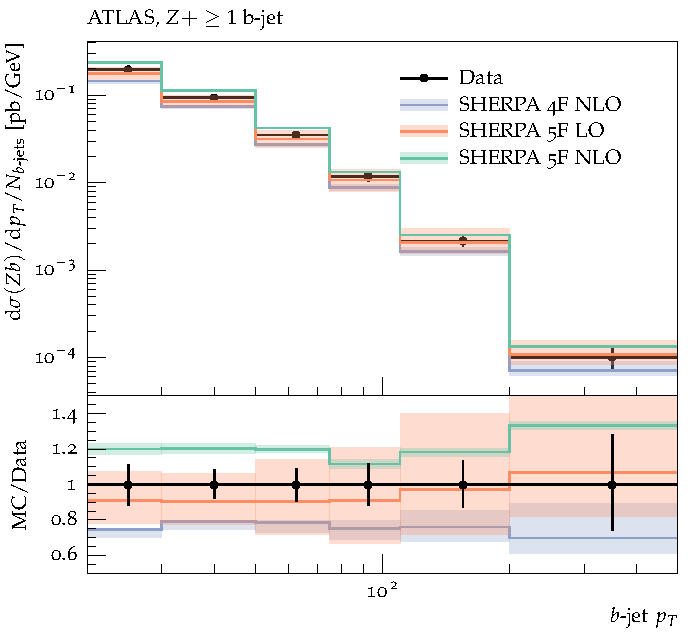
\includegraphics[scale=0.5]{figs/zbb/d03-x01-y01.pdf} 
   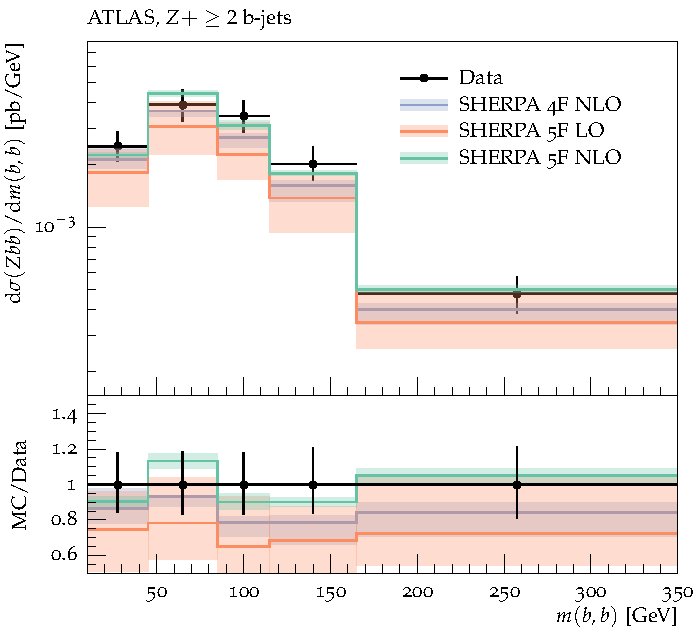
\includegraphics[scale=0.5]{figs/zbb/d23-x01-y01.pdf} 
\end{figure}
\begin{figure}[htbp]
   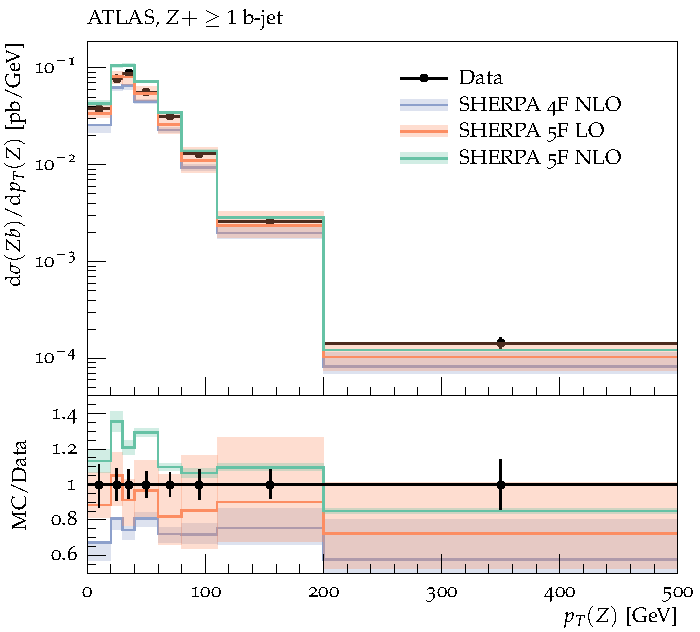
\includegraphics[scale=0.5]{figs/zbb/d15-x01-y01.pdf} 
   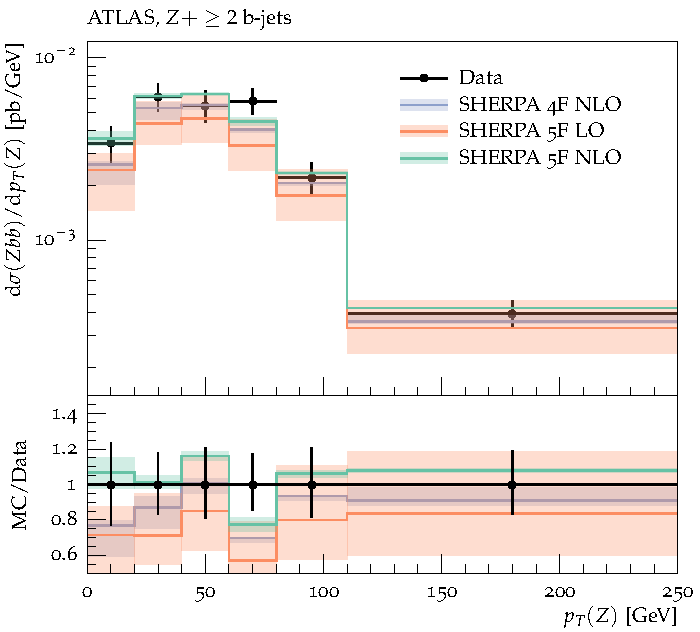
\includegraphics[scale=0.5]{figs/zbb/d25-x01-y01.pdf} 
\end{figure}
\begin{figure}[htbp]
   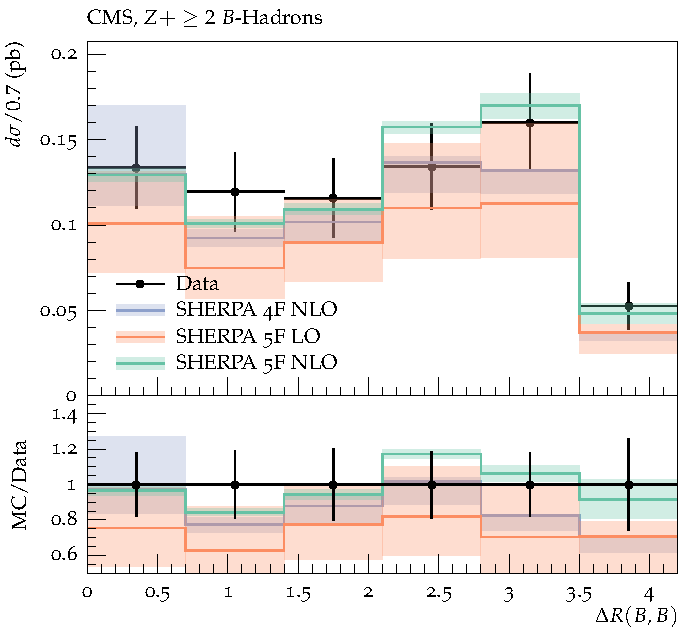
\includegraphics[scale=0.5]{figs/zbb/d01-x01-y01.pdf} 
   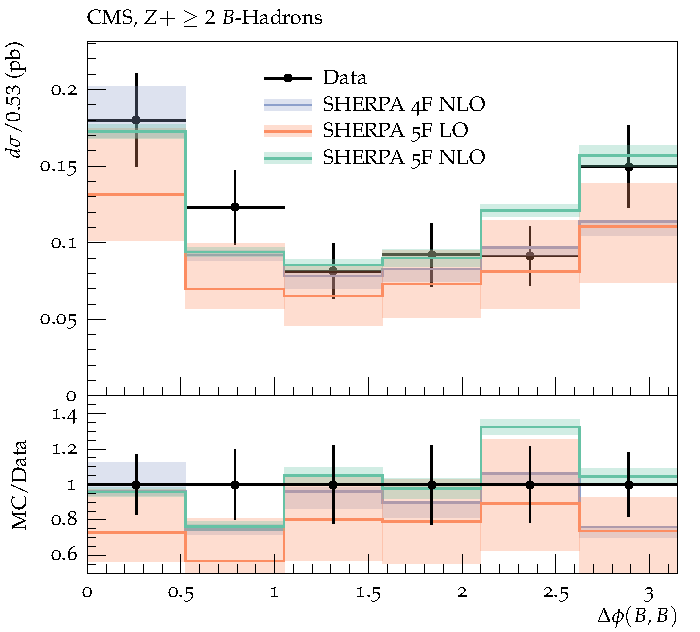
\includegraphics[scale=0.5]{figs/zbb/d02-x01-y01.pdf} 
\end{figure}
\subsubsection{Z+b 4F rescaled results}
...4F \MCatNLO rescaled to MCFM...
\begin{figure}[htbp]
   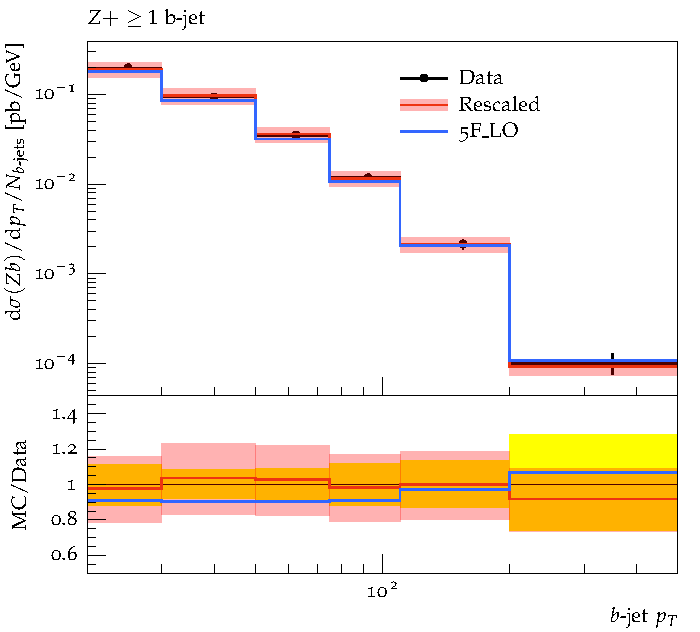
\includegraphics[scale=0.5]{figs/zbb/d03-x01-y01_rescaled.pdf} 
   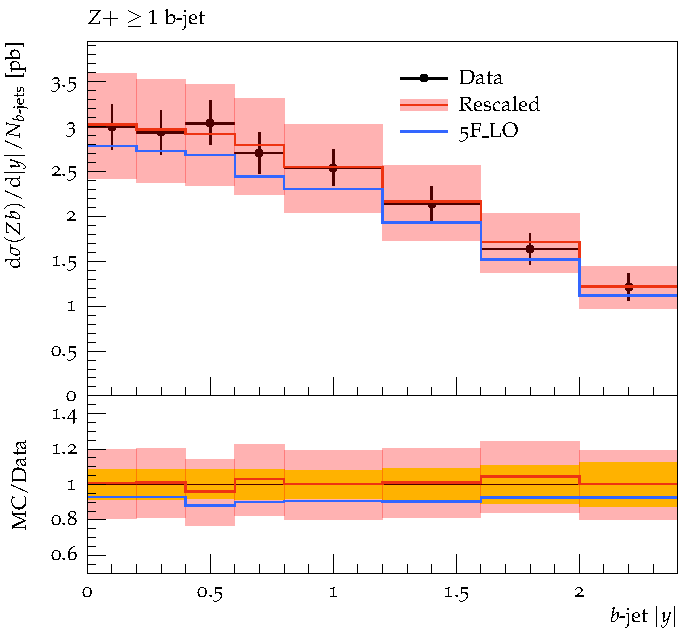
\includegraphics[scale=0.5]{figs/zbb/d05-x01-y01_rescaled.pdf} 
\end{figure}
\begin{figure}[htbp]
   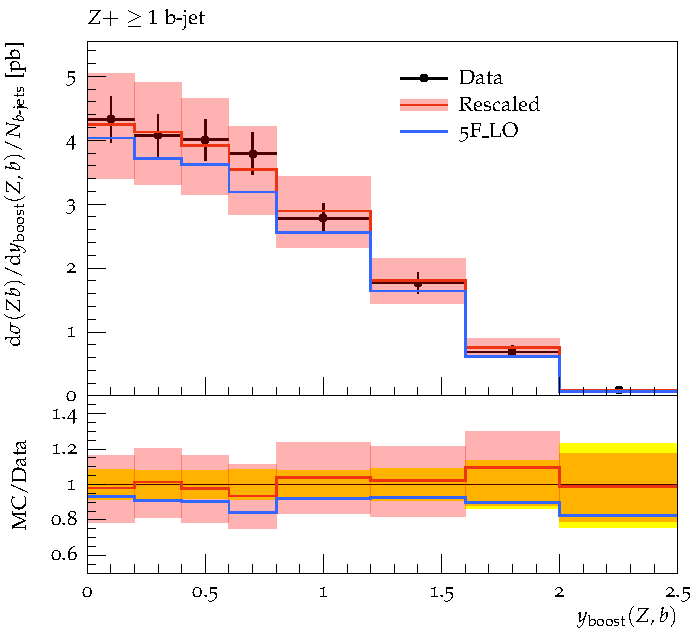
\includegraphics[scale=0.5]{figs/zbb/d07-x01-y01_rescaled.pdf} 
   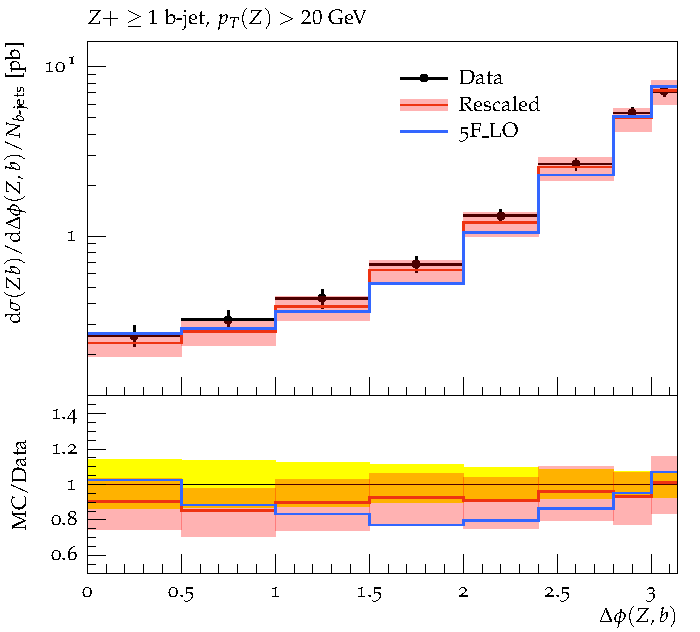
\includegraphics[scale=0.5]{figs/zbb/d11-x01-y01_rescaled.pdf} 
\end{figure}
\begin{figure}[htbp]
   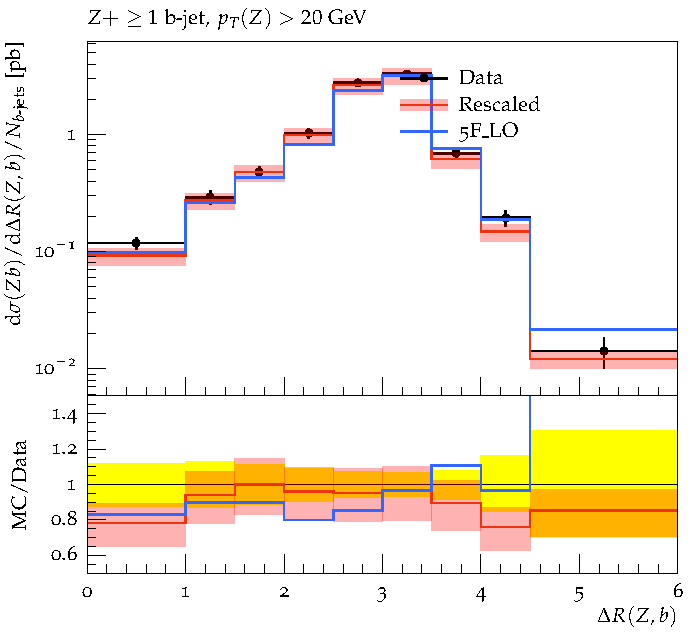
\includegraphics[scale=0.5]{figs/zbb/d13-x01-y01_rescaled.pdf} 
\end{figure}

\subsection{W+b production with \Sherpa}
\begin{figure}[htbp]
   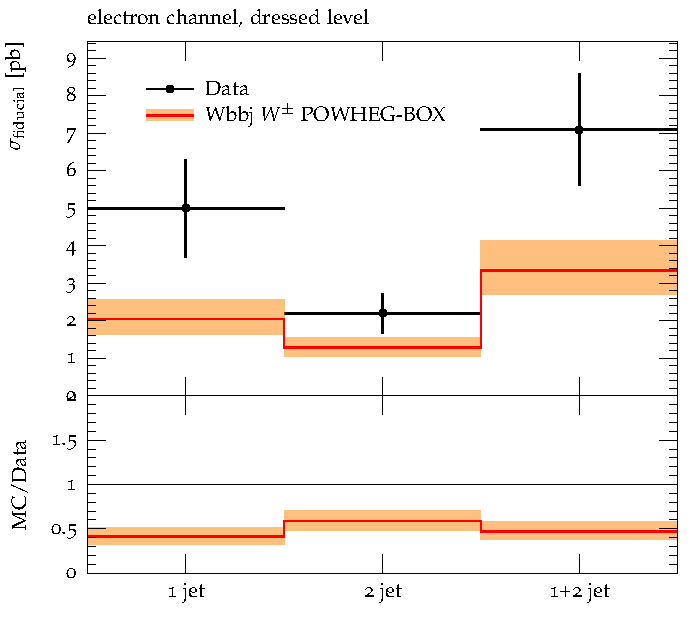
\includegraphics[scale=0.5]{figs/wbb/d01-x01-y01.pdf}
\end{figure}

\begin{figure}[htbp]
   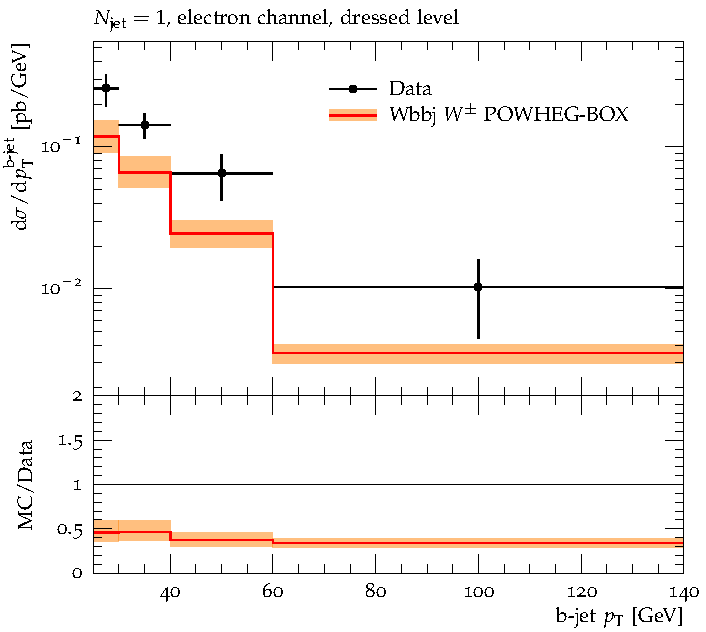
\includegraphics[scale=0.5]{figs/wbb/d02-x01-y01.pdf}
   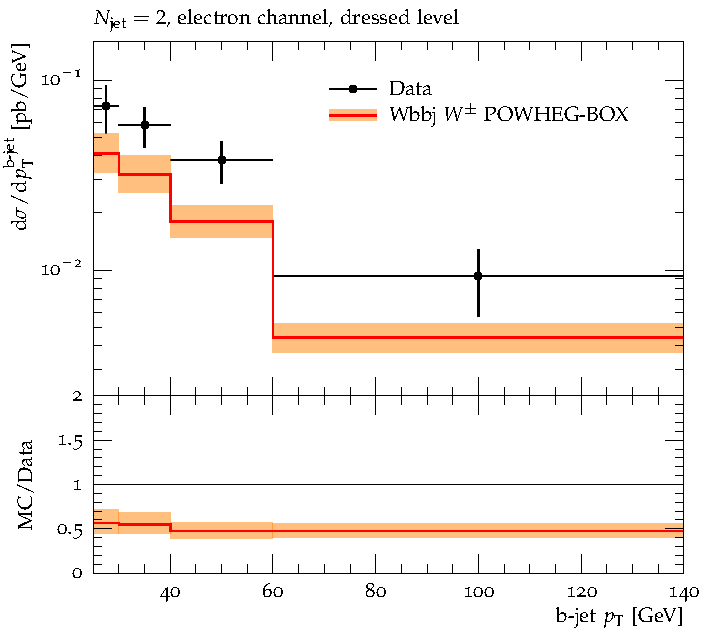
\includegraphics[scale=0.5]{figs/wbb/d02-x02-y01.pdf}
\end{figure}

\subsection{Z+b(b) production with \Herwig}
\label{sec:ZHerwig}

\subsubsection{Z+b, 5F}

\subsubsection{Z+bb, 5F}

\subsubsection{Z+bb, 4F}

\subsection{W+bb production with \Herwig}
\label{sec:WHerwig}

\subsubsection{W+bb, 4F}

\subsection{Conclusions}

\bibliography{vbb}

\end{document}
